\subsection{Photon Generation}
In order to trace photons into the scene we need a method of creating photons, this is implemented in the light defintion,
each light object has a associated function that will produce a random photon from the light that is consitent with the
type of light, for instance a point light will generate a photon with origin exactlu at the origin of the light source and
in a random direction, an area light produces a photon with origin on the area of the light with direction taken from a
cosine weighted hemisphere distribution in the direction of the normal of the light. Each photon that is emitted from the
light sources begin with the full power of the light source, this will be scaled by the number of emitted photons after
all photons have been gathered.

\subsection{Photon Emission(3 pages)}
Once the scene data has been created it is passed to the back-end, the first step that is performed is photon gathering,
in this stage photons are emmited from all light sources in the scene and are stored in one of the photon maps for use
in the raytracing stage of the algoithm, as discussed in the design chapter the emission of the photons is performed in
parralell using pthreads, each thread is started with a data structure that contains the scene into which the photons
are being emmited from and the number of photons the thread is responsible for storing in the photon map, for each photon
that is to be stored we write to a queue that is read by the main thread. along with the photon traced a summary of the
path of the photon is written in the queue. Once all of the photons have been emitted a flag is set to inform that the
thread is finished, this is sent along the same channel as the photons. The number of photons that are emmited is determined
by the power of each of the lights, as a result lights with higher power will have more photons emitted for that light as
we need to be able to calculate the contribution from these light sources with more accuracy than lights with lower power
as they contribure more to the illuminaion of the scene.

\subsection{Russian Roulette}
When a traced photon intersects with an object in the scene we must make a decision as to what will happen to the photon,
this could be one of specular reflection or transmission, diffuse reflection or absorbtion, the desicion is performed
by creating a uniform variable \todo{Add Epsilony thing here}, given reflection, transmission and diffuse coefficients
$\rho_{s}, \rho_{t}, \rho_{d}$ we can create a distribution of photon emittion (Figure~\ref{fig:rr_dist}) we then take
a uniform variable $\xi$ in the range [0, 1) 

\begin{figure}
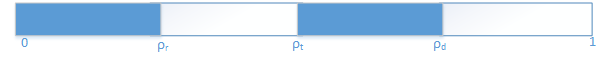
\includegraphics{./images/russian_roulette_distribution.png}
\label{fig:rr_dist}
\caption{Russian roulette distribution}
\end{figure}

\subsection{Photon Power}
In the above distribution we assume that the reflectance coefficients are a single number, in our syste, this is not
the case as we have a coefficient for each of thr RGB colour channels, when performing the russian roulette calculation
we use the average reflectance of each of the components, the case for the specuar coefficient is given below.

\begin{equation}
\rho_s = \frac{\rho_s^r + \rho_s^g + \rho_s^b}{3}
\end{equation}

As a result of using average reflectance we need to scale the power of the photons that are traced in order to keep the
radiance estimate at the limit correct.

\begin{equation}
\begin{array}{lcr} \Phi_s^r = \Phi_s^r * \frac{\rho_s^r}{\rho_{s}}\\ \Phi_s^g = \Phi_s^g * \frac{\rho_s^g}{\rho_{s}}\\ \Phi_s^b = \Phi_s^b * \frac{\rho_s^b}{\rho_{s}}
\end{array}
\end{equation}

As discussed in \todo{Jensen Citation} at each interaction with a non-specular surface the power of the reflected photon
needs to be scaled by the reflectance of the surface, this would insert many low power into the photon map, he suggests
using monte carlo sampling and russian roulette to create a photon with probablilty proportional to the reflectance
of the surface.

Storing the photons is performed at each interaction with a non specular surface, the reason for not storing at specular
surface is that specular BRDFs contain the dirac delta function as a result the photon map cannot be used to evaluate the
radiance at this point, we use traditional raytracing to perform the radiance at specular surfaces.

\subsection{Volume Photon Map}
When tracing the photons through the scene and it intersects with a participating media we begin by transmitting the
photon into the media based on the surface properties of the media, after this we iterativly scatter the photon in the
media storing the photon at each of the points of scattering, the scattering is determined by the scattering and
absorbtion coefficients of the media, the media has a component for each of the colour components, when moving through
the volume the power of the photon is reduced much like the reduction for reflections at surfaces, like surfaces this
would end with many low power photons in the map instead we perform importance sampling by modifiing the distance that
the photon moves through the media inbetween interactions with the media, equation \todo{Add the fucntion and a citation}
is used for the importance sampling. At each interaction of the participating media the photon can either be absorbed
or scattered, this is determined by the albedo $\Lambda$ \todo{Give Albedo Function}

\missingfigure{Volume Photon Map}

\begin{figure}
\centering
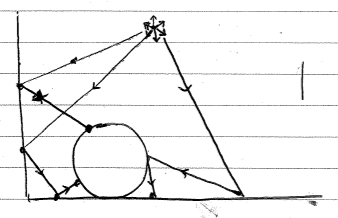
\includegraphics{./images/photon_mapping.png}
\label{fig:surface_photon_map}
\caption{Surface photon map}
\end{figure}

\begin{figure}
\begin{lstlisting}
struct thread_output_data
{
	char last      : 1;
	char diffuse   : 1;
	char specular  : 1;
	char light     : 5;
	union
	{
		photon_t photon;
		int      emitted;
	};
};
\end{lstlisting}
\caption{Output of photon emittion threads}
\end{figure}

\subsubsection{Algorithmic Overview}
%
%\begin{algorithm}[h!]
%	\KwData{Scene Description}
%	\KwResult{Photon paps for input scene}
%	\For{each light in scene}
%	{
%		TracePhoton(photon);
%	}
%	\caption{Photon mapping algothm}
%\end{algorithm}
%
%\begin{algorithm}[h!]
%	\KwData{Scene Description, Photon}
%	\KwResult{Photon added to photon map}
%	\eIf{photon intersects scene}
%	{
%	
%	}
%	{
%		Discard photon;
%	}
%\caption{TracePhoton}
%\end{algorithm}

\subsection{Photon Data Structure (0.5 page)}
As noted by Jensen \todo{cite} the need for a compact representation of the individual photons in the photon map is vital
as it is typical for their to be many thousands to millions of photons in order to perform accurate radiance estimates,
the initial implementation of the photon map included a naive implementation that used double width floating point values.
\todo{Analysis for speed}

\subsection{K-D Tree Balancing (1 page)}
When performing radiance estimations with the photon map we will be performing nearest neighbour searches on points within
the map, this requires the photon map to be arrainged in a manner such that this search can be performed efficiently.
In order to do this we store the photon map in a left-balanced k-d tree. A left balanced tree is a tree structure where
at each level of the tree the depth of the children differs by at most one, \todo{finish the explination of the LEFT balanced tree}
this allows us to store the photon map in an array with the location of the children in the photon map known implicitly,
for a photon in position $i$ the children of the photon can be found at the $(2i + 1)^{th}$ and $(2i + 2)^{th}$
location for the left and right tree respectivly.

\missingfigure{KDBalance Algorithm}
\todo{Add the median of median algorithm here}

\begin{figure}
\centering
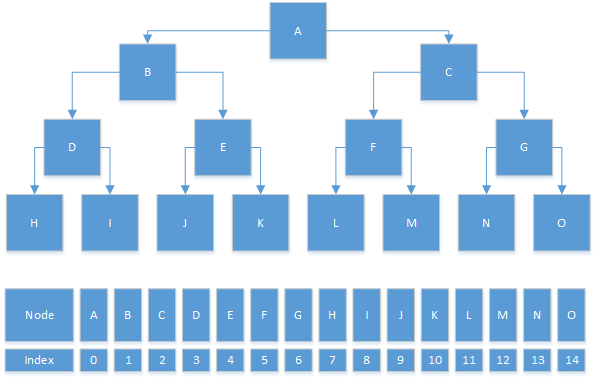
\includegraphics[scale=0.75]{./implementation/left-balanced-tree.png}
\caption{Left balanced tree and its memory layout}
\end{figure}

\subsection{Selection Statistic}
During the balancing procedure we need to partition the tree such that half the elements are less than the median
this can be seen as finding the $i/2^{th}$ largest element in the list, this can be performed in linear time by using
the median of medians algorithm \todo{cite}. Below is a comparison for the runnning time of the balancing procedure for
the nieve selection algorithm and the median of medians algorithm. As we are left-balancing the tree we also cannot
just take the median of the data, we must adjust the median such that the left half of the tree will fill before the right.

\missingfigure{times for median of median compared}

\subsection{Photon Termination}
During the photon tracing stage at each of the intersections that are found we must make a choice whether to refect absorb or transmit
the photon, for purely specular materials the choice is simple, that is we will reflect the photon. For materials that are not purely
specular such as diffuse materials the choice is less clear, we must take into account the BDRF of the material.
